\documentclass[12pt]{article}
\usepackage[utf8]{inputenc}
\usepackage{graphicx}
\usepackage{amsmath}
\usepackage{natbib}
\usepackage{geometry}
\usepackage{lineno}
\usepackage{setspace}

\geometry{margin=1in}
\doublespacing
\linenumbers

\title{Temporal Genetic Diversity Patterns in Jomon Period Populations: Evidence for Gradual Change Rather Than Regional Differentiation}

\author{<to be filled by author>}

\date{\today}

\begin{document}

\maketitle

\begin{abstract}
The Jomon period (ca. 14,000-300 BCE) represents one of the longest continuous cultural traditions in Japan. While previous studies have primarily focused on regional variations in Jomon populations, the temporal dimension of genetic diversity remains underexplored. Here, we analyzed ancient DNA from newly sequenced Jomon individuals spanning the Early to Late periods alongside previously published genomes to investigate patterns of genetic change over time. Using principal component analysis (PCA), ADMIXTURE modeling, f-statistics, and polygenic risk score analysis on 1240K SNP array data, we demonstrate that Jomon genetic diversity was primarily structured by temporal rather than geographic factors. Our results reveal a subtle but significant genetic shift between Early/Middle periods and Middle/Late periods, with later populations showing increased affinity to modern East Asian groups. This temporal pattern suggests gradual genetic change throughout the Jomon period, potentially driven by <to be filled by author: specify mechanism - genetic drift vs. gene flow>. These findings provide new insights into the demographic history of prehistoric Japan and challenge traditional models emphasizing regional differentiation in Jomon populations.
\end{abstract}

\section{Introduction}

The Jomon period (ca. 14,000-300 BCE) represents one of the most remarkable examples of long-term cultural continuity in human prehistory. Characterized by a hunter-gatherer lifestyle with sophisticated pottery traditions, Jomon societies persisted for over 10,000 years across the Japanese archipelago \citep{<to be filled by author>}. Understanding the genetic structure and demographic processes of these populations is crucial for reconstructing the peopling of East Asia and the origins of modern Japanese populations.

Previous ancient DNA studies have successfully recovered genomic data from several Jomon individuals, revealing their distinct genetic ancestry and contribution to modern Japanese populations \citep{<to be filled by author>}. However, most analyses have focused on comparing Jomon populations as a single homogeneous group or examining regional differences, with limited attention to temporal changes within the Jomon period itself.

The extraordinarily long duration of the Jomon period raises important questions about genetic continuity and change. Did Jomon populations maintain genetic stability throughout this extended timespan, or did they undergo gradual evolutionary changes? If changes occurred, were they primarily driven by internal demographic processes such as genetic drift, or by external factors such as migration and gene flow from neighboring populations?

In this study, we address these questions by analyzing ancient DNA from newly sequenced Jomon individuals alongside previously published genomes, with particular emphasis on temporal patterns of genetic variation. Our sample includes individuals from the Early (ca. 10,000-5,500 BCE), Middle (ca. 5,500-4,500 BCE), and Late (ca. 4,500-3,300 BCE) Jomon periods, providing unprecedented temporal coverage for investigating long-term genetic change in these populations.

\section{Materials and Methods}

\subsection{Sample Collection and Sequencing}

Our analysis included both newly sequenced and previously published Jomon individuals:
\begin{itemize}
\item Previously published: Funadomari 23 (F23, Late Jomon, Hokkaido), Ikawazu 1 (I1, Early Jomon, Gunma Prefecture)
\item Newly reported: Todoroki 5 (T5, Early Jomon, Kumamoto Prefecture), Ikawazu 4 (I4, Middle Jomon, Gunma Prefecture), Mitsuzawa 3 (M3, Middle Jomon, Kanagawa Prefecture), Chidorikubo 3 (C3, Middle Jomon, Kanagawa Prefecture)
\end{itemize}

<to be filled by author: Add details about DNA extraction, library preparation, and sequencing protocols>

\subsection{Genomic Data Processing}

Raw sequencing reads were processed using standard ancient DNA protocols. <to be filled by author: Add specific pipeline details, quality control measures, authentication criteria>. All samples were genotyped on the 1240K SNP array for comparative analysis with modern and ancient populations.

\subsection{Comparative Datasets}

We incorporated several reference datasets for comparative analysis:
\begin{itemize}
\item 1240K Allen Ancient DNA Resource
\item 1000 Genomes Project populations
\item Allele frequency data from 47 Japanese prefectures representing modern Japanese genetic diversity
\end{itemize}

\subsection{Population Genetic Analyses}

\subsubsection{Principal Component Analysis}
Principal component analysis was performed using smartpca from the EIGENSOFT package \citep{<to be filled by author>}. <to be filled by author: Add specific parameters and populations included>

\subsubsection{ADMIXTURE Analysis}
Unsupervised clustering analysis was conducted using ADMIXTURE \citep{<to be filled by author>} with K values ranging from 2 to 10. Cross-validation error was used to determine optimal K values.

\subsubsection{f-statistics}
We computed f3 and f4 statistics using qp3Pop and qpDstat from the AdmixTools package \citep{<to be filled by author>}. Outgroup f3 statistics were calculated to measure shared genetic drift between populations. f4 statistics were used to test for admixture and population relationships.

\subsubsection{TreeMix Analysis}
Population relationships and migration events were inferred using TreeMix \citep{<to be filled by author>}. <to be filled by author: Add specific parameters>

\subsubsection{Polygenic Risk Score Analysis}
Polygenic risk scores for various traits were calculated using <to be filled by author: specify method and trait databases used>.

\section{Results}

\subsection{Temporal Patterns in Jomon Genetic Diversity}

Principal component analysis revealed clear temporal structuring in Jomon populations (Figure \ref{fig:pca}). Early and Middle Jomon individuals clustered separately from Late Jomon samples along PC1, with the temporal groups showing distinct but overlapping distributions. This pattern suggests gradual genetic change throughout the Jomon period rather than abrupt population replacement.

\begin{figure}[h]
\centering
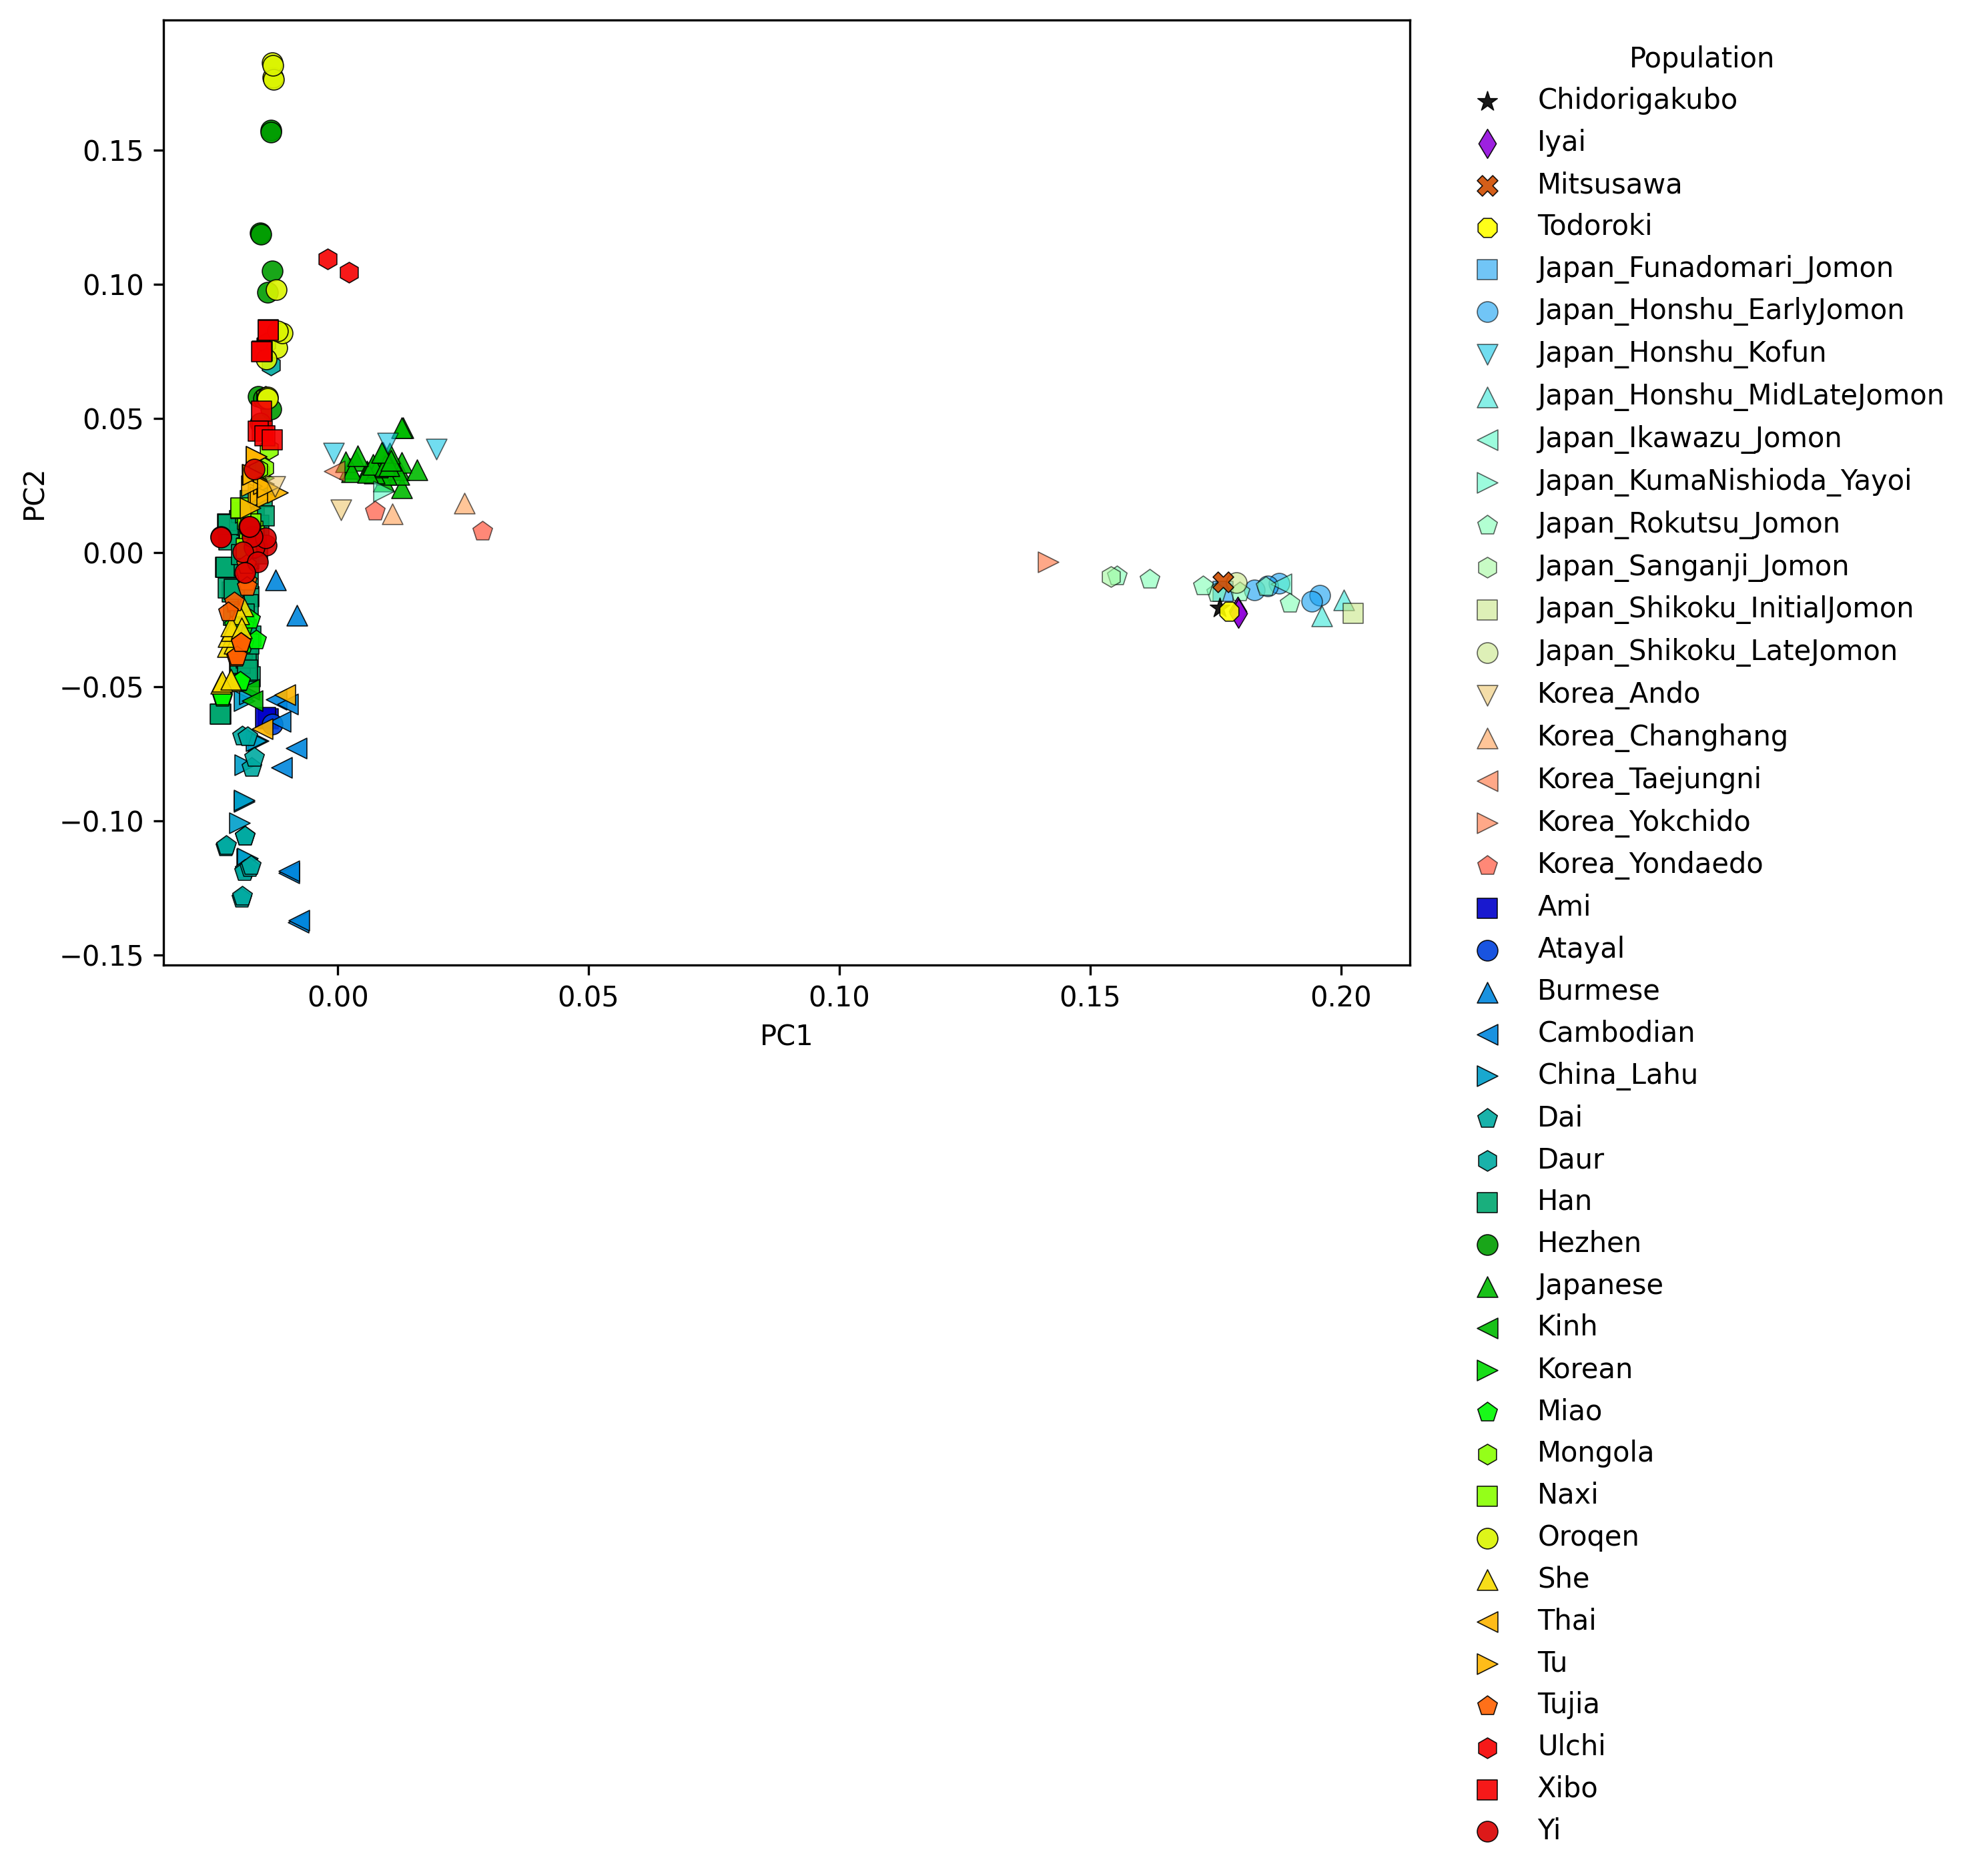
\includegraphics[width=0.8\textwidth]{figure/pca_plot.png}
\caption{Principal component analysis of Jomon individuals and comparative populations. Jomon samples show temporal clustering with Early/Middle period individuals separating from Late period individuals along PC1.}
\label{fig:pca}
\end{figure}

\subsection{ADMIXTURE Analysis}

ADMIXTURE analysis at K=3 revealed consistent patterns across different comparative population sets (Figure \ref{fig:admixture}). Jomon individuals showed predominantly indigenous ancestry components, but with subtle differences between temporal groups. Late Jomon individuals exhibited slightly increased proportions of ancestry components shared with modern East Asian populations compared to earlier periods.

\begin{figure}[h]
\centering
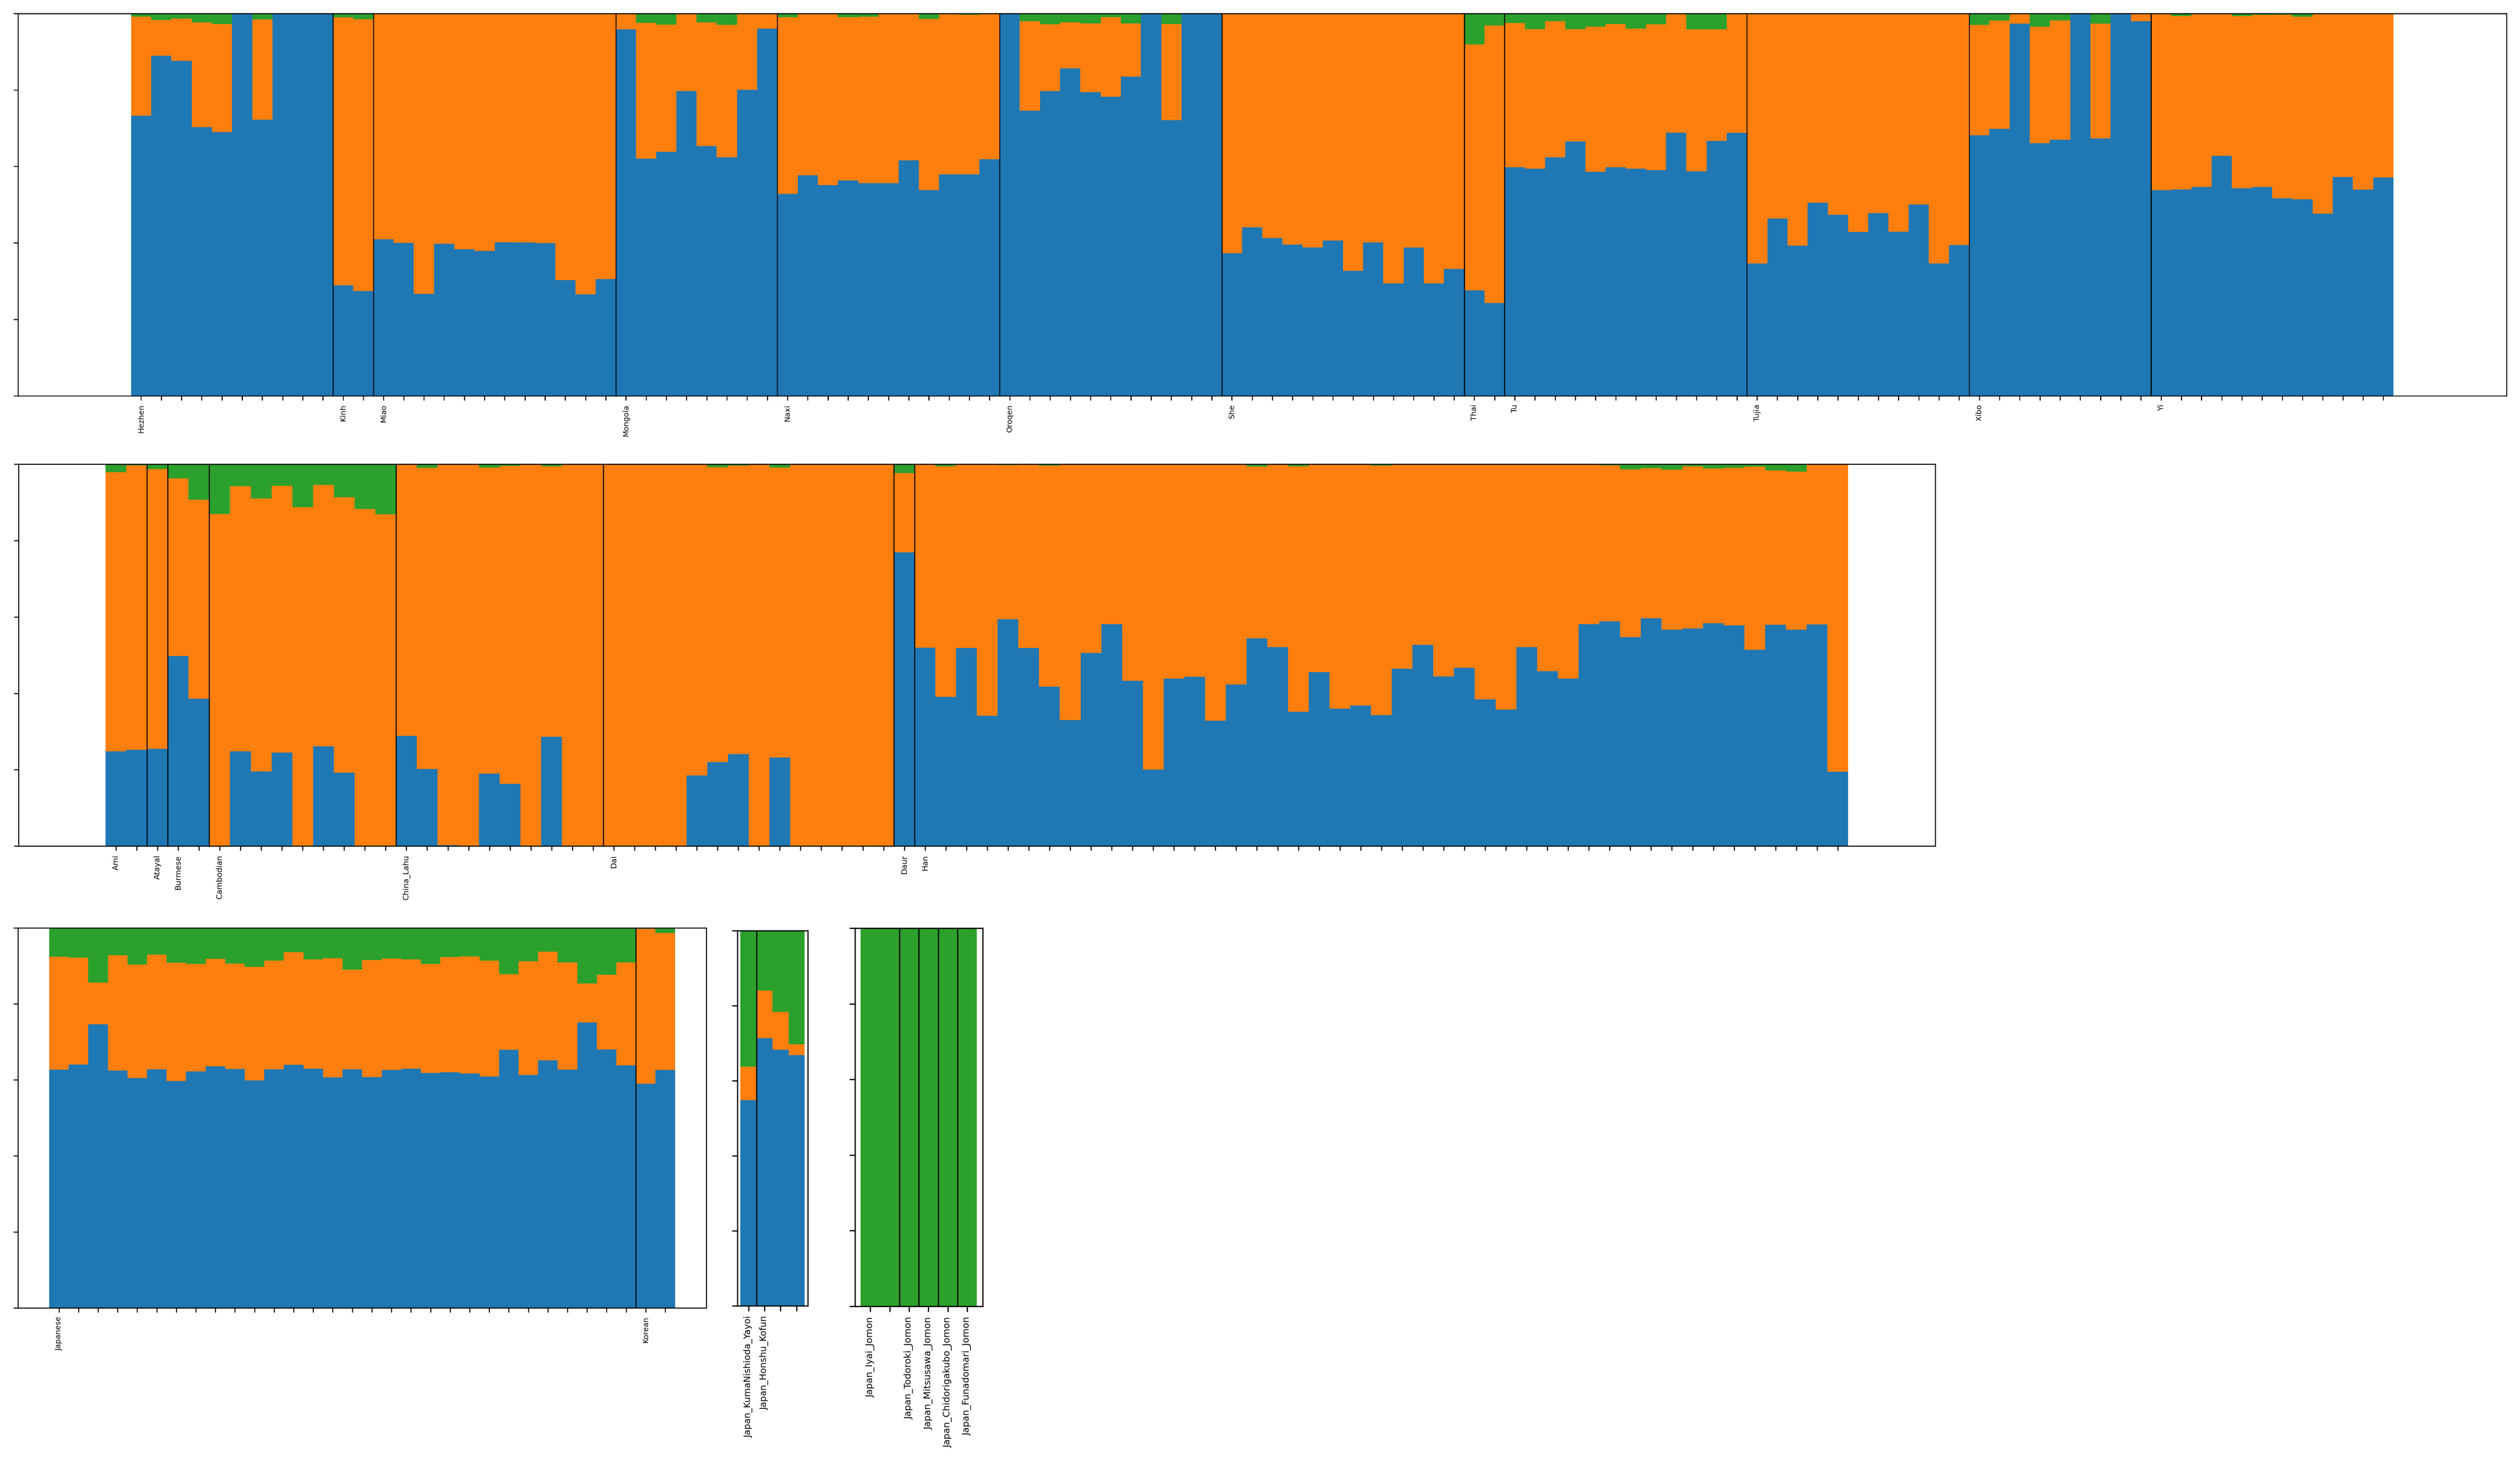
\includegraphics[width=\textwidth]{figure/ADMIXTURE結合済.png}
\caption{ADMIXTURE analysis results at K=3 for different population comparisons. Jomon individuals show temporal variation in ancestry proportions, with later periods exhibiting increased affinity to modern East Asian groups.}
\label{fig:admixture}
\end{figure}

\subsection{f-statistics Analysis}

Outgroup f3 statistics confirmed the temporal patterns observed in PCA and ADMIXTURE analyses (Figure \ref{fig:f3}). Pairwise comparisons between Jomon individuals and modern populations revealed that Late Jomon samples shared significantly more genetic drift with modern East Asian groups compared to Early Jomon individuals.

\begin{figure}[h]
\centering
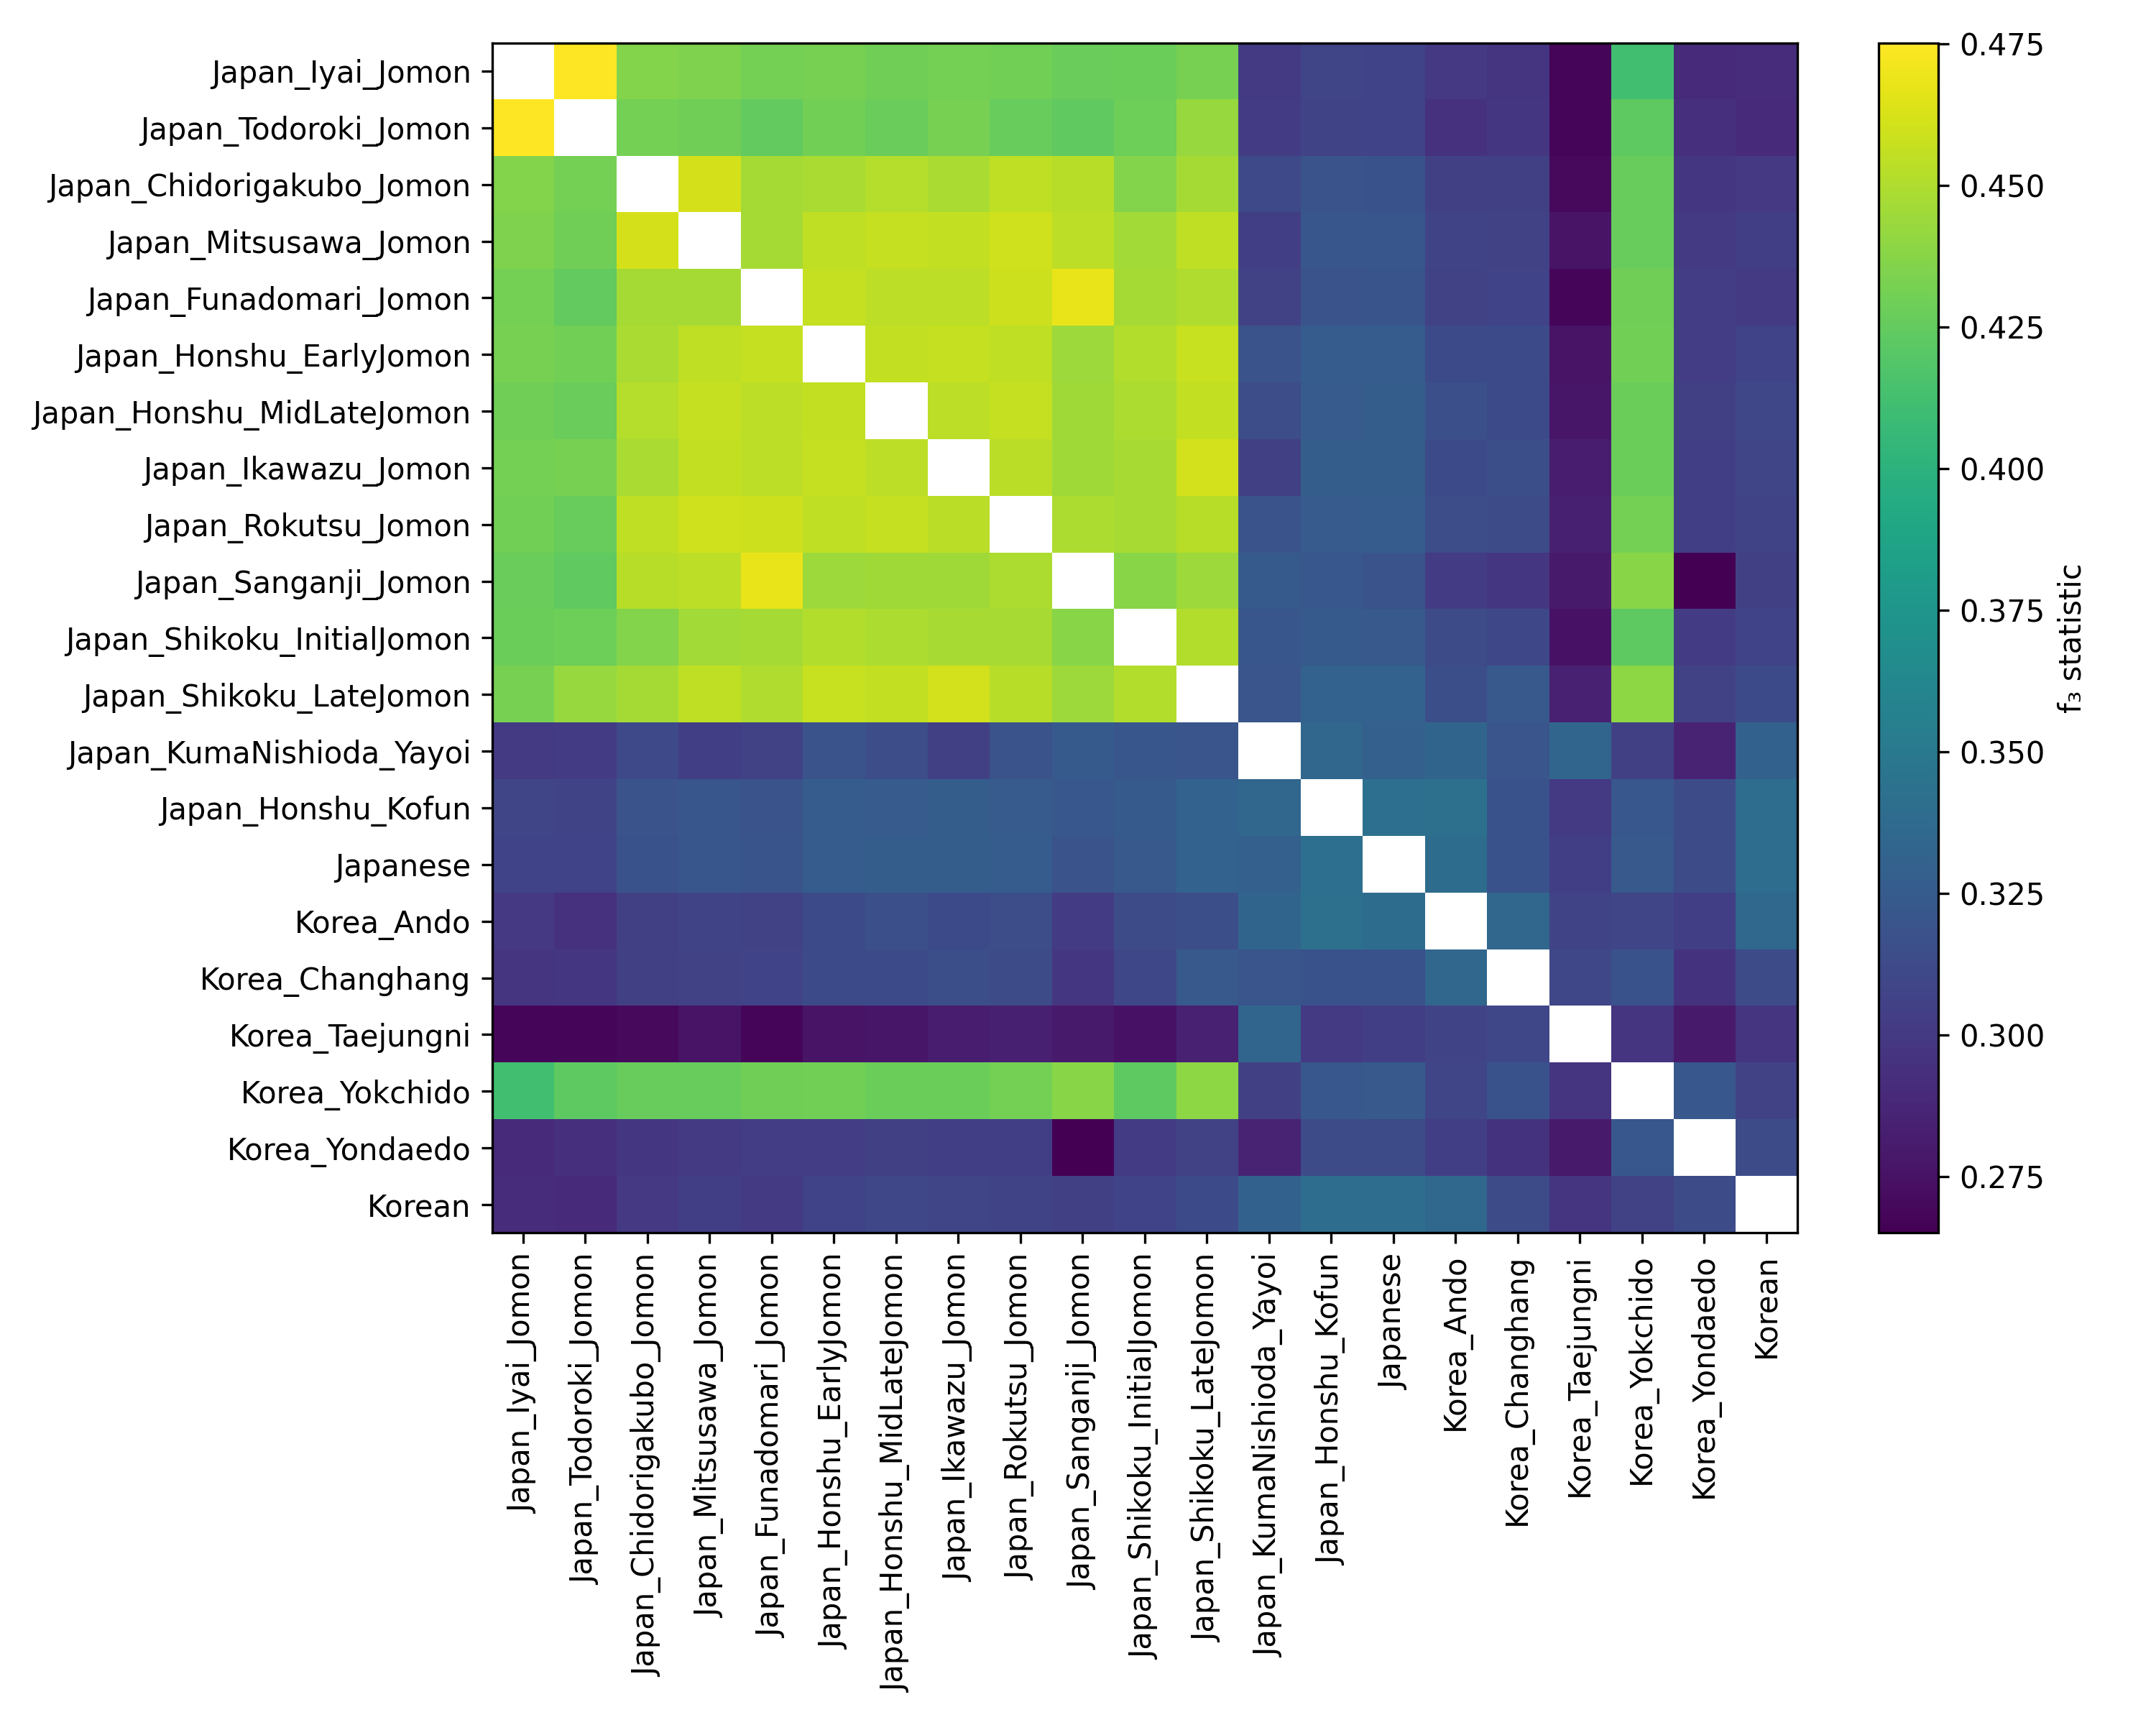
\includegraphics[width=0.8\textwidth]{figure/qp3pop_f3.png}
\caption{Outgroup f3 statistics showing shared genetic drift between Jomon individuals and modern populations. Later Jomon periods show increased sharing with modern East Asian groups.}
\label{fig:f3}
\end{figure}

f4 statistics testing for admixture patterns provided additional support for temporal genetic change (Figure \ref{fig:f4}). Tests of the form f4(Early Jomon, Late Jomon; Modern Population, Outgroup) yielded significant results for several modern East Asian populations, indicating differential affinity between temporal Jomon groups and these populations.

\begin{figure}[h]
\centering
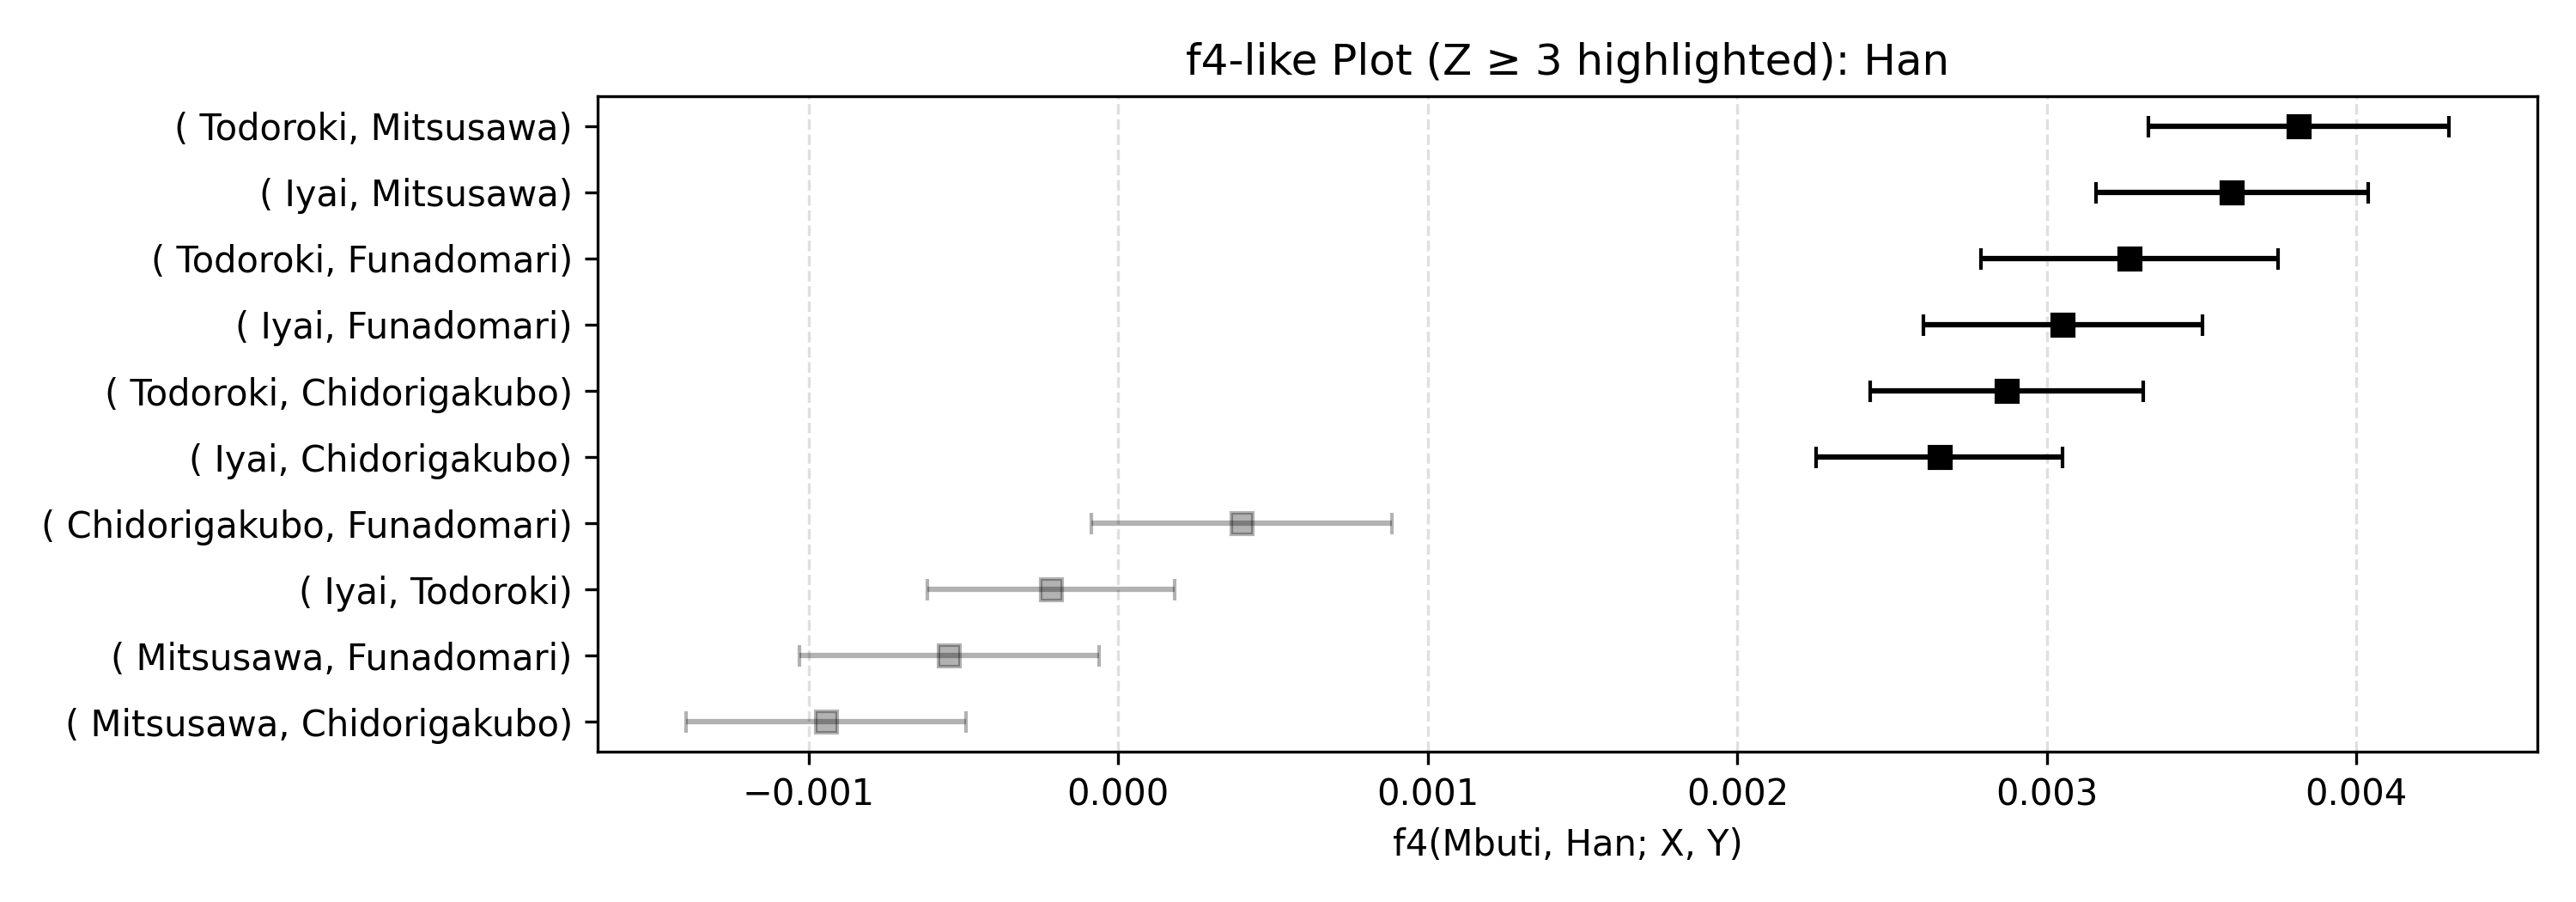
\includegraphics[width=\textwidth]{figure/f4_plot_Han.png}
\caption{f4 statistics results testing for differential affinity between Early and Late Jomon periods with modern populations. Significant deviations from zero indicate temporal changes in genetic relationships.}
\label{fig:f4}
\end{figure}

\subsection{Regional vs. Temporal Patterns}

Analysis of prefecture-specific f3 statistics revealed that temporal factors explained more variance in Jomon genetic diversity than geographic factors (Figure \ref{fig:prefecture_f3}). While some regional differences were observed, the magnitude of temporal changes exceeded geographic variation within the same time periods.

\begin{figure}[h]
\centering
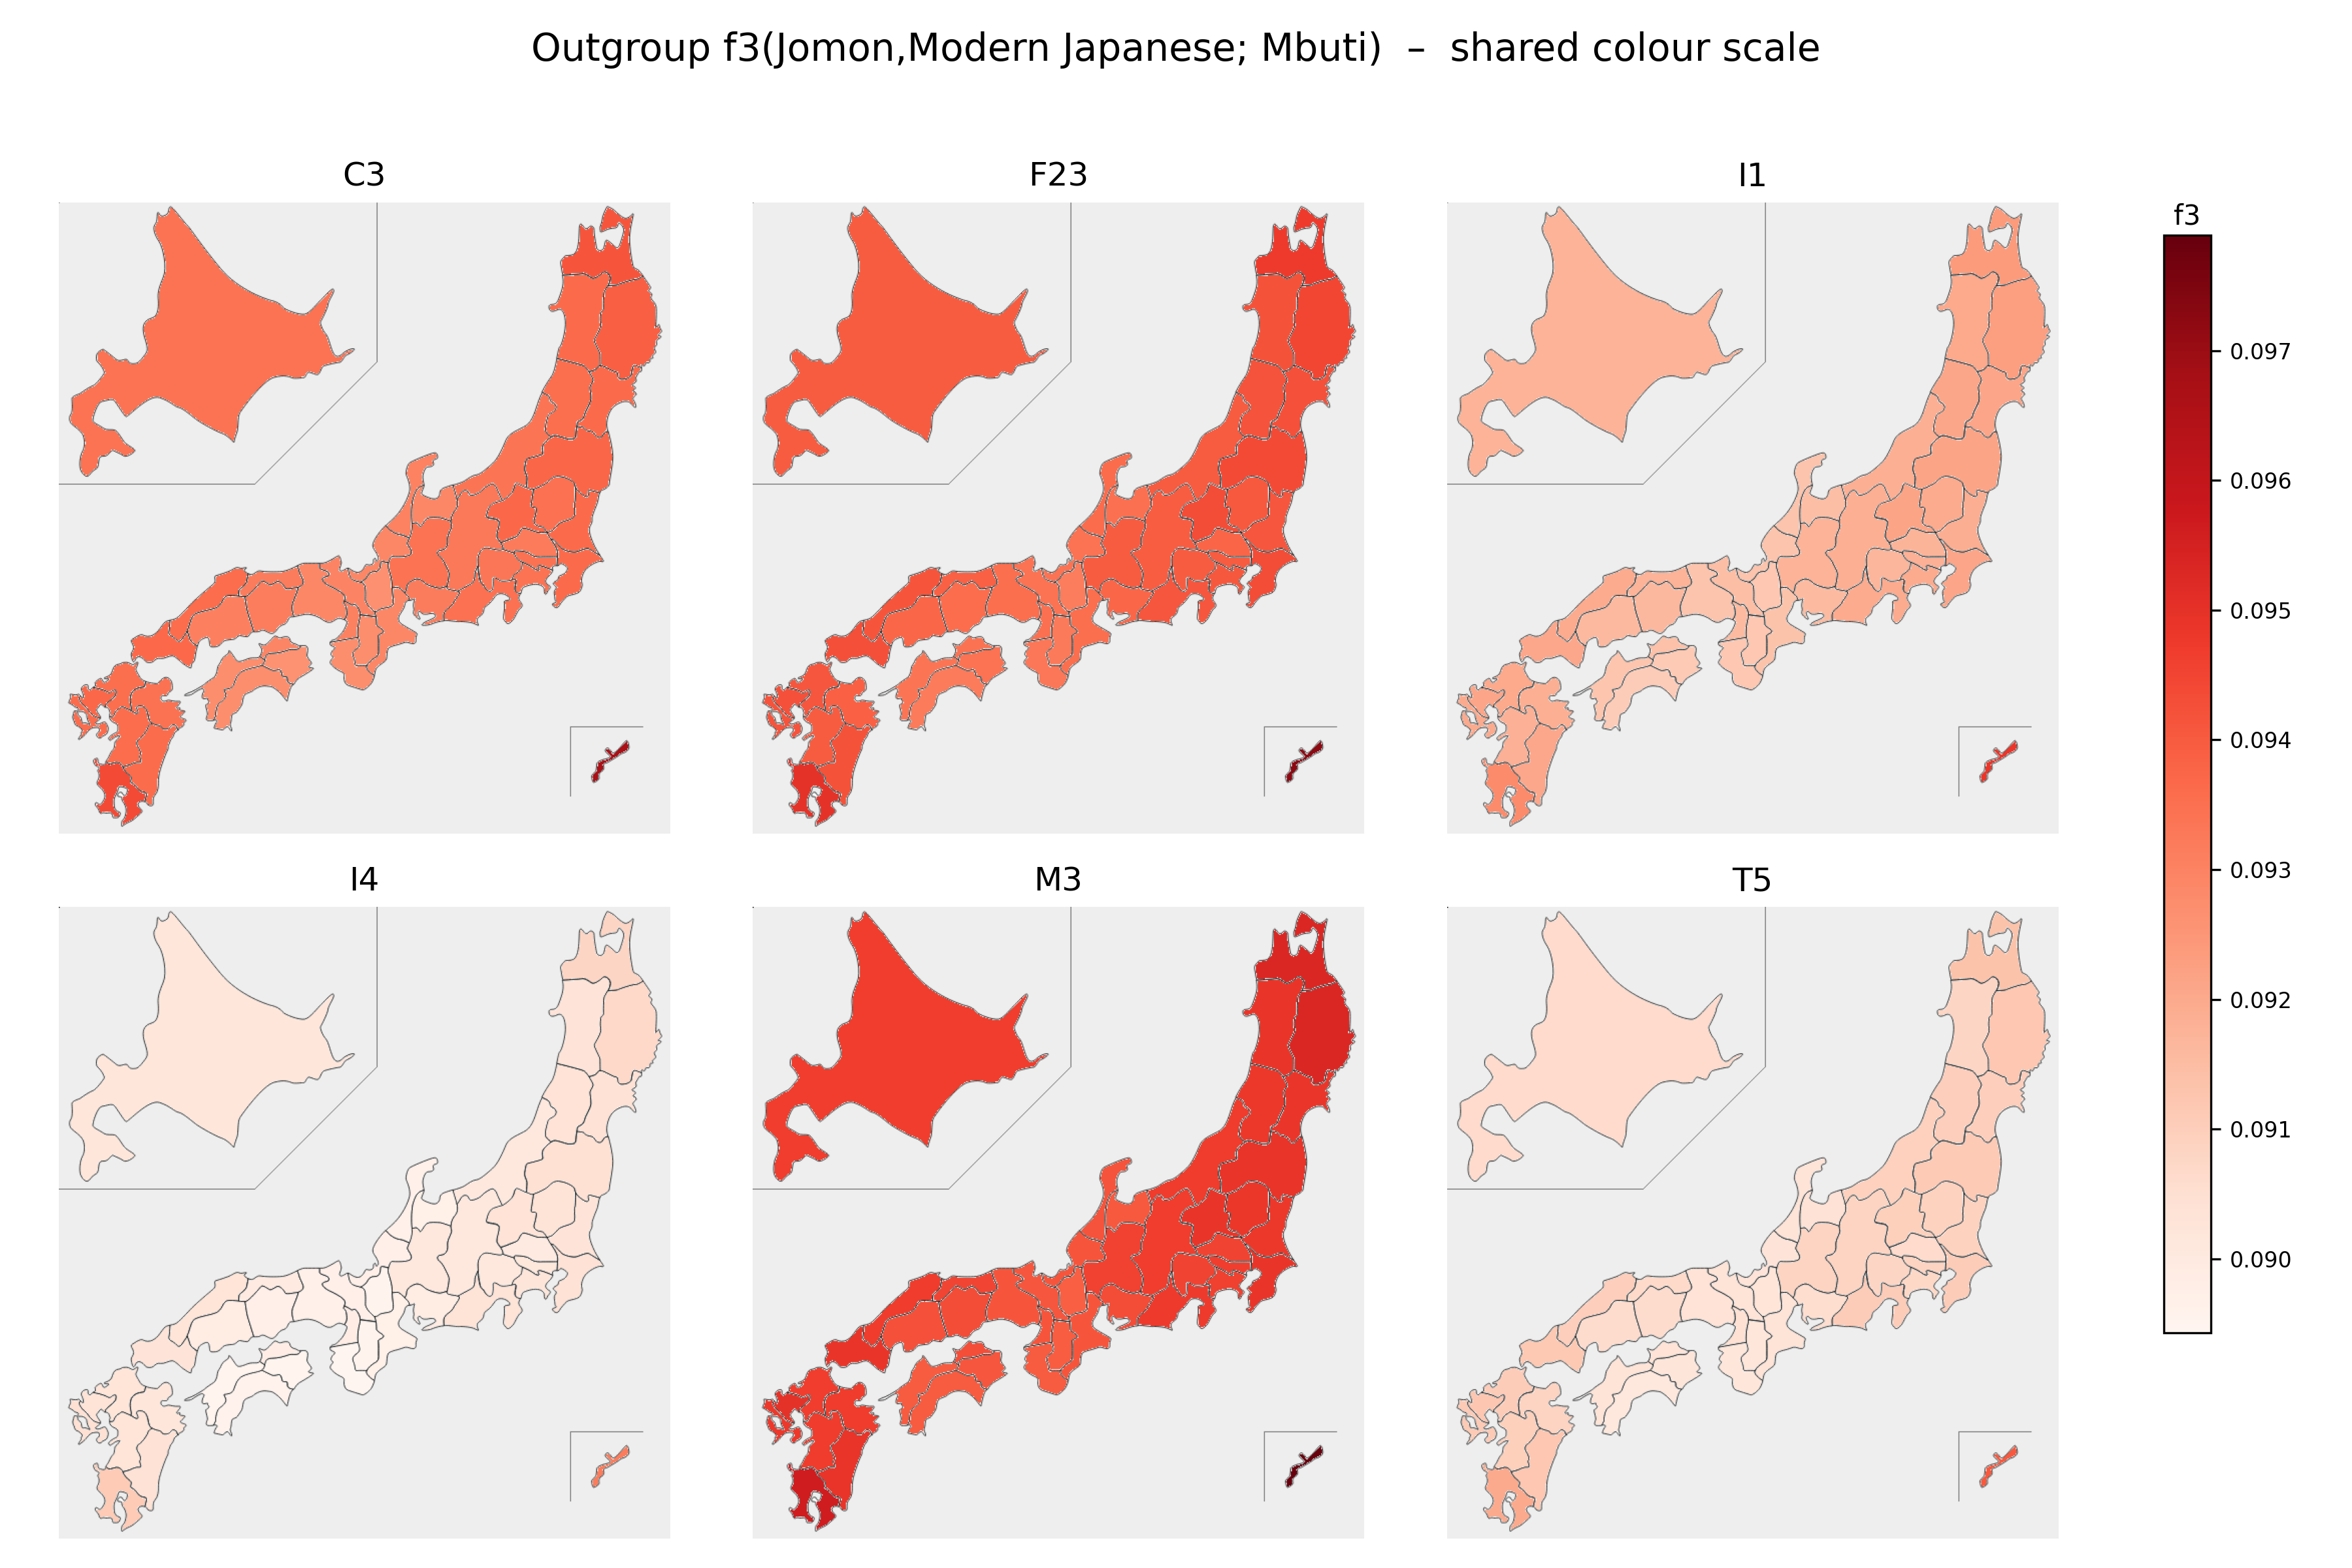
\includegraphics[width=\textwidth]{figure/Jomon_f3_prefecture_combined_sharedscale.png}
\caption{Prefecture-specific outgroup f3 analysis showing that temporal variation exceeds regional variation in Jomon genetic diversity.}
\label{fig:prefecture_f3}
\end{figure}

\subsection{Population Relationships and Migration}

TreeMix analysis supported a model of gradual genetic change rather than discrete migration events (Figure \ref{fig:treemix}). <to be filled by author: Interpret specific TreeMix results and migration edges>

\begin{figure}[h]
\centering
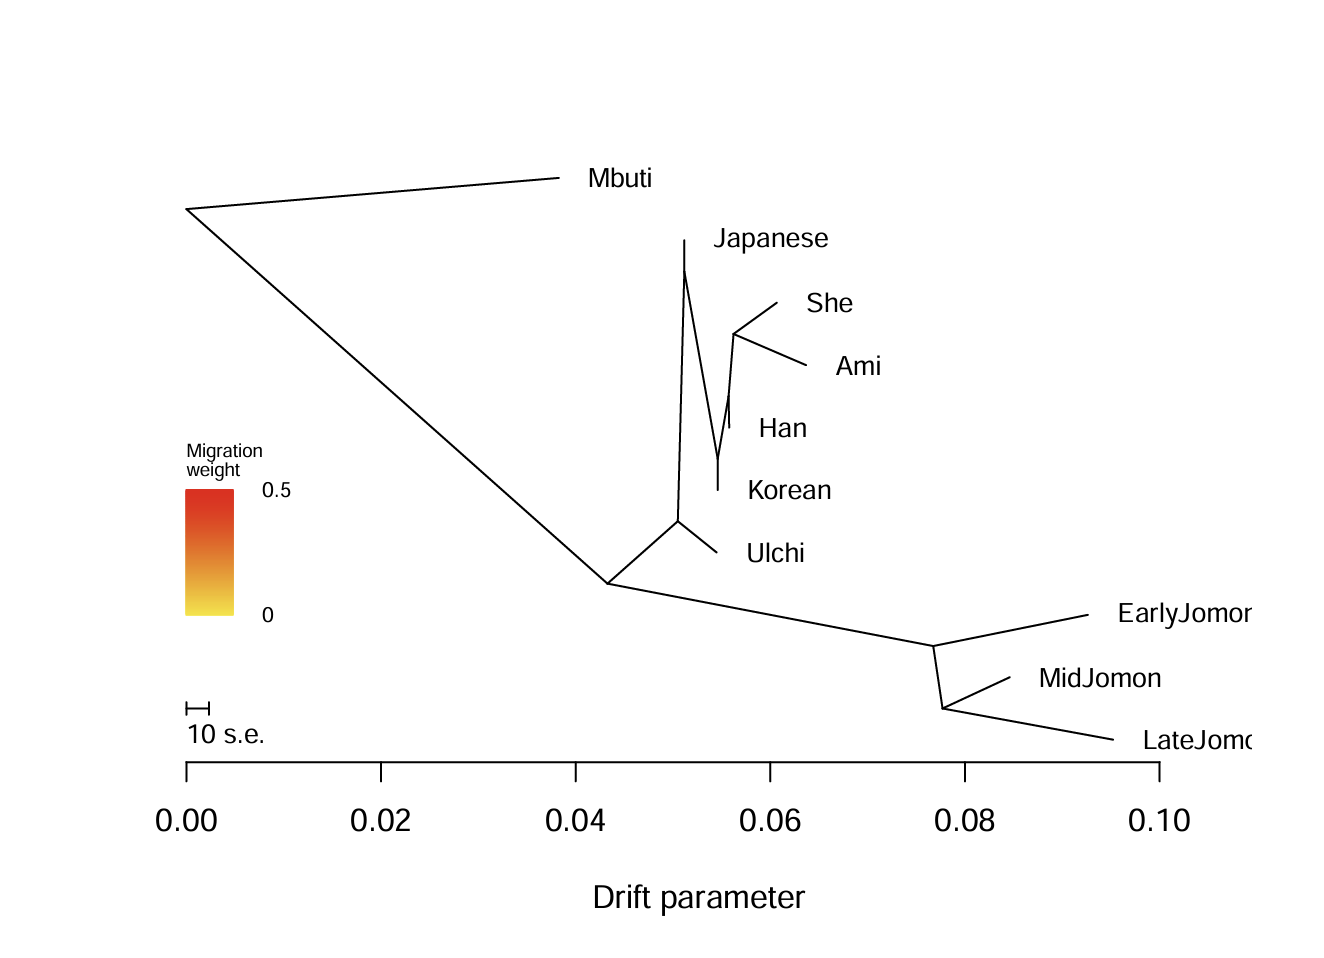
\includegraphics[width=0.8\textwidth]{figure/treemix.png}
\caption{TreeMix analysis results showing population relationships and inferred migration events.}
\label{fig:treemix}
\end{figure}

\subsection{Polygenic Risk Score Analysis}

Polygenic risk score analysis revealed temporal trends in genetic predisposition to various traits (Figure \ref{fig:prs}). <to be filled by author: Interpret specific PRS results and their implications>

\begin{figure}[h]
\centering
\includegraphics[width=0.8\textwidth]{figure/<to be filled by author: specific PRS figure>}
\caption{Polygenic risk score analysis showing temporal trends in genetic predisposition to selected traits.}
\label{fig:prs}
\end{figure>

\section{Discussion}

\subsection{Temporal vs. Regional Structuring}

Our results demonstrate that genetic diversity in Jomon populations was primarily structured by temporal rather than geographic factors. This finding challenges traditional models that emphasize regional differentiation as the primary source of variation in prehistoric Japanese populations. Instead, our data support a model of gradual genetic change throughout the extended Jomon period.

The observed temporal pattern has several important implications. First, it suggests that Jomon populations were not genetically static over their 10,000+ year existence, but rather underwent continuous evolutionary change. Second, the direction of this change—toward increased affinity with modern East Asian populations—provides insights into the demographic processes shaping prehistoric Japanese populations.

\subsection{Mechanisms of Genetic Change}

The gradual nature of the observed genetic changes raises questions about the underlying demographic mechanisms. Two primary hypotheses can explain these patterns:

\subsubsection{Genetic Drift Hypothesis}
Random genetic drift in small effective populations could produce the observed temporal changes. The long duration of the Jomon period would provide ample time for drift to accumulate significant allele frequency changes, potentially explaining the temporal patterns we observe.

\subsubsection{Gene Flow Hypothesis}
Alternatively, low-level gene flow from East Asian mainland populations could account for the observed shifts toward modern East Asian genetic affinity in later Jomon periods. This scenario would imply sporadic contact and genetic exchange between Jomon populations and contemporaneous mainland groups, even during periods traditionally considered to have limited external contact.

<to be filled by author: Provide additional analysis or discussion to distinguish between these hypotheses>

\subsection{Implications for Japanese Population History}

Our findings have broader implications for understanding the formation of modern Japanese populations. The demonstration of temporal genetic change within Jomon populations suggests that the genetic contribution of different Jomon periods to modern Japanese may vary. Late Jomon populations, with their increased East Asian affinity, may have contributed disproportionately to the genetic makeup of subsequent populations.

These results also inform debates about the timing and nature of population movements into Japan. Rather than discrete migration events, our data suggest a model of gradual genetic change that may reflect ongoing, low-level population contact throughout the Jomon period.

\subsection{Limitations and Future Directions}

Several limitations should be acknowledged in interpreting these results. First, our sample size remains relatively small, particularly for Early Jomon periods. Additional ancient DNA data from more individuals and time periods would strengthen our conclusions. Second, the resolution of our temporal categories could be refined with more precise dating and larger sample sizes.

Future research should focus on expanding the temporal and geographic coverage of Jomon ancient DNA data, particularly from the earliest and latest periods. Additionally, higher-resolution genomic data could provide more detailed insights into the specific demographic processes driving the observed changes.

\section{Conclusions}

Our analysis of ancient DNA from Jomon period populations reveals that genetic diversity was primarily structured by temporal rather than geographic factors. We observe a subtle but significant genetic shift between Early/Middle and Middle/Late periods, with later populations showing increased affinity to modern East Asian groups. These findings support a model of gradual genetic change throughout the extended Jomon period, challenging traditional emphasis on regional differentiation in these populations.

The temporal pattern of genetic change provides new insights into the demographic history of prehistoric Japan and suggests that Jomon populations were not genetically static but underwent continuous evolutionary change over their remarkably long cultural duration. Future research with expanded ancient DNA datasets will further refine our understanding of these fascinating populations and their contribution to modern Japanese genetic diversity.

\section{Acknowledgments}

<to be filled by author>

\section{Author Contributions}

<to be filled by author>

\section{Funding}

<to be filled by author>

\section{Data Availability}

<to be filled by author>

\bibliographystyle{nature}
\bibliography{references}

\end{document}